 \documentclass{article}
\usepackage[utf8]{inputenc}
\usepackage[a4paper, total={7in, 10in}]{geometry}
\usepackage{braket}
\usepackage{xcolor}
\usepackage{amsmath}
\usepackage{amssymb}
\usepackage{amsfonts}
\usepackage{graphicx}
\usepackage{svg}
\usepackage{float}
\usepackage{tikz}
\usepackage[ruled,vlined]{algorithm2e}
\usepackage{multicol}
\usepackage[backend=biber,style=alphabetic,sorting=ynt]{biblatex}
\usepackage{xcolor}
%\addbibresource{sample.bib} %Import the bibliography file

\newcommand{\commentt}[1]{\textcolor{blue}{ \textbf{[COMMENT]} #1}}
\newcommand{\ctt}[1]{\commentt{#1}}
\newcommand{\prb}[1]{ \mathbf{Pr} \left[ {#1} \right]}
\newcommand{\onotation}[1]{\(\mathcal{O} \left( {#1}  \right) \)}
\newcommand{\ona}[1]{\onotation{#1}}
\newcommand{\PSI}{{\ket{\psi}}}
\newcommand{\LESn}{\ket{\psi_n}}
\newcommand{\LESa}{\ket{\phi_n}}
\newcommand{\LESs}{\frac{1}{\sqrt{n}}\sum_{i}{\ket{\left(0^{i}10^{n-i}\right)^{n}}}}
\newcommand{\Hn}{\mathcal{H}_{n}}
\newcommand{\Ep}{\frac{1}{\sqrt{2^n}}\sum^{2^n}_{x}{ \ket{xx}}}
\newcommand{\HON}{\ket{\psi_{\text{honest}}}}
\newcommand{\Lemma}{\paragraph{Lemma.}}


\setlength{\columnsep}{0.6cm}

\newcommand{\Gz}{ G_{z}^{\delta} } 

\begin{document}

\title{Quantum LTC With Positive Rate}
\author{David Ponarovsky}
\maketitle
%\begin{multicols*}{2}
\newcommand{ \Hw }{ \delta\Delta -\Delta^{\frac{1}{2}-\varepsilon}/\delta  }
	\newcommand{ \Nw }{ \Delta^{\frac{3}{2}-\varepsilon}} 
	  \newcommand{ \Gu } { \Gamma^{\cup} }
	  \newcommand{ \Guq } { \Gamma^{\cup, \square} }

    	\newcommand{ \Gsa } {\Gamma_{\square_{1}} }
	\newcommand{ \Gsb } {\Gamma_{\square_{2}} }
        \newcommand{ \Aa } { C_{A_{1}}}  
	\newcommand{ \Ab } { C_{A_{2}}}
	\newcommand{ \Ac } { C_{A_{3}}}
	\newcommand{ \Aab } { \Aa \otimes \Ab } 
	\newcommand{ \Aac } { \Aa \otimes \Ac }
	\newcommand{ \Aabc } { \Aa \otimes \Ab \otimes \Ac }
	\newcommand{ \Aabp } { \Aa^{\perp} \otimes \Ab^{\perp} } 
	\newcommand{ \Aacp } { \Aa^{\perp} \otimes \Ac^{\perp} }
	\newcommand{ \Aabcp } { \Aa^{\perp} \otimes \Ab^{\perp} \otimes \Ac^{\perp} }
	\newcommand{ \Aabpp } { \left( \Aabp \right)^\perp } 
	\newcommand{ \Aacpp } { \left( \Aacp \right)^\perp }
	\newcommand{ \Aabcpp } { \left( \Aabcp \right)^\perp }
	\newcommand{ \YY } {  y_{1}y_{2}^{\top} }
	\newcommand{ \ZZ } {  z_{1}z_{2}^{\top} } 
	\newcommand{ \TT } { \tilde{\tau} } 


  \paragraph{preamble.} preamble.  
  \begin{figure}[H]
            %\label{fig:square}
            \begin{center}
            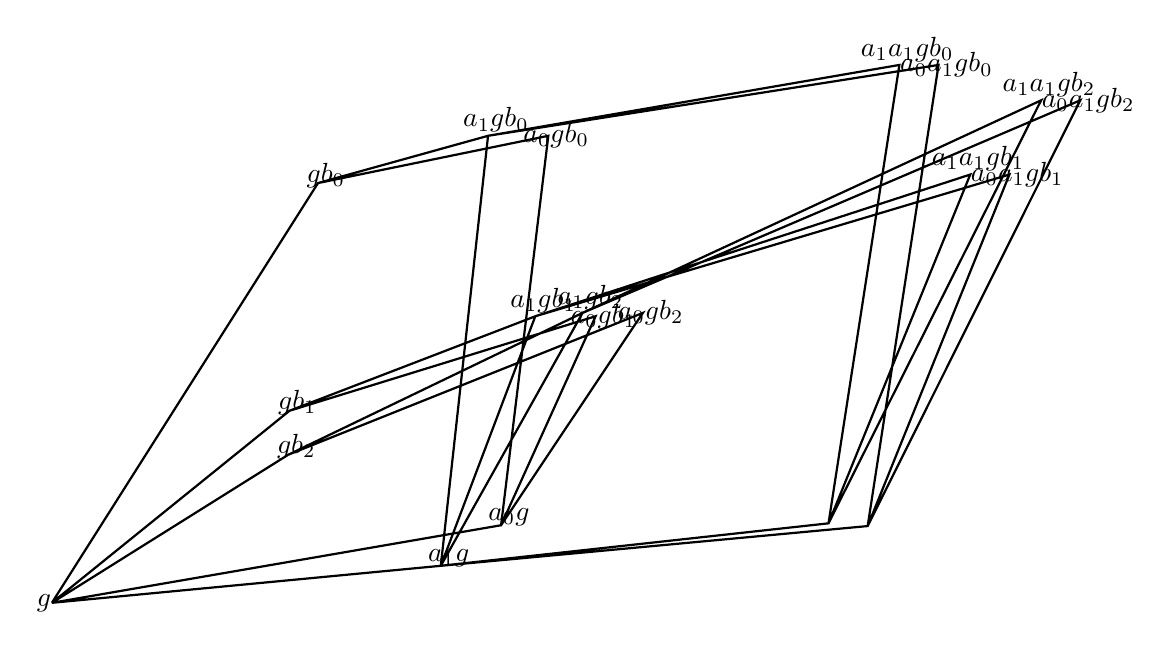
\begin{tikzpicture}
            \draw[thick](0,0)(0, 0) -- (3.3801444639622344,5.330941981780722) -- (6.304895010214057,5.930941981780721) -- (5.704895010214058,0.9851683897888519) -- (0, 0)
(0, 0) -- (3.0178397476658327,2.4390675578834173) -- (6.904895010214058,3.6390675578834175) -- (5.704895010214058,0.9851683897888519) -- (0, 0)
(0, 0) -- (3.0037982492898663,1.8816420823575566) -- (7.5048950102140575,3.6816420823575564) -- (5.704895010214058,0.9851683897888519) -- (0, 0)
(0, 0) -- (3.3801444639622344,5.330941981780722) -- (5.539491408544737,5.930941981780721) -- (4.939491408544737,0.4701138342996021) -- (0, 0)
(0, 0) -- (3.0178397476658327,2.4390675578834173) -- (6.139491408544737,3.6390675578834175) -- (4.939491408544737,0.4701138342996021) -- (0, 0)
(0, 0) -- (3.0037982492898663,1.8816420823575566) -- (6.739491408544737,3.6816420823575564) -- (4.939491408544737,0.4701138342996021) -- (0, 0)
(4.939491408544737, 0.4701138342996021) -- (5.539491408544737,5.930941981780721) -- (11.260676210527304,6.830941981780722) -- (10.360676210527304,0.9747120918902664) -- (4.939491408544737, 0.4701138342996021)
(4.939491408544737, 0.4701138342996021) -- (6.139491408544737,3.6390675578834175) -- (12.160676210527305,5.439067557883417) -- (10.360676210527304,0.9747120918902664) -- (4.939491408544737, 0.4701138342996021)
(4.939491408544737, 0.4701138342996021) -- (6.739491408544737,3.6816420823575564) -- (13.060676210527305,6.381642082357557) -- (10.360676210527304,0.9747120918902664) -- (4.939491408544737, 0.4701138342996021)
(4.939491408544737, 0.4701138342996021) -- (5.539491408544737,5.930941981780721) -- (10.763245208864692,6.830941981780722) -- (9.863245208864692,1.0094556236420666) -- (4.939491408544737, 0.4701138342996021)
(4.939491408544737, 0.4701138342996021) -- (6.139491408544737,3.6390675578834175) -- (11.663245208864693,5.439067557883417) -- (9.863245208864692,1.0094556236420666) -- (4.939491408544737, 0.4701138342996021)
(4.939491408544737, 0.4701138342996021) -- (6.739491408544737,3.6816420823575564) -- (12.563245208864693,6.381642082357557) -- (9.863245208864692,1.0094556236420666) -- (4.939491408544737, 0.4701138342996021)
;
\node at (6.404895010214057,5.930941981780721) {$ a_{ 0  } gb_{ 0 } $};
\node at (7.0048950102140575,3.6390675578834175) {$ a_{ 0  } gb_{ 1 } $};
\node at (7.604895010214057,3.6816420823575564) {$ a_{ 0  } gb_{ 2 } $};
\node at (5.639491408544736,6.130941981780722) {$ a_{ 1  } gb_{ 0 } $};
\node at (6.239491408544737,3.8390675578834177) {$ a_{ 1  } gb_{ 1 } $};
\node at (6.8394914085447365,3.8816420823575566) {$ a_{ 1  } gb_{ 2 } $};
\node at (11.360676210527304,6.830941981780722) {$ a_{ 0  } a_{ 1 }gb_{ 0 } $};
\node at (12.260676210527304,5.439067557883417) {$ a_{ 0  } a_{ 1 }gb_{ 1 } $};
\node at (13.160676210527305,6.381642082357557) {$ a_{ 0  } a_{ 1 }gb_{ 2 } $};
\node at (10.863245208864692,7.030941981780722) {$ a_{ 1  } a_{ 1 }gb_{ 0 } $};
\node at (11.763245208864692,5.6390675578834175) {$ a_{ 1  } a_{ 1 }gb_{ 1 } $};
\node at (12.663245208864693,6.581642082357557) {$ a_{ 1  } a_{ 1 }gb_{ 2 } $};
\node at (-0.1,0) {$ g $};
\node at (5.804895010214057,1.085168389788852) {$ a_{ 0 }g $};
\node at (5.039491408544737,0.570113834299602) {$ a_{ 1 }g $};
\node at (3.4801444639622345,5.430941981780721) {$ gb_{ 0 } $};
\node at (3.117839747665833,2.5390675578834174) {$ gb_{ 1 } $};
\node at (3.1037982492898664,1.9816420823575567) {$ gb_{ 2 } $};

            \end{tikzpicture}
            \end{center}
            \caption{Square of the complex, with edges $(g,ag), (agb, gb) \in E_A,
            (g,gb), (agb, ag) \in E_B.$ \label{fig:square}
            }
            \end{figure}
 \begin{figure}[H]
            %\label{fig:square}
            \begin{center}
            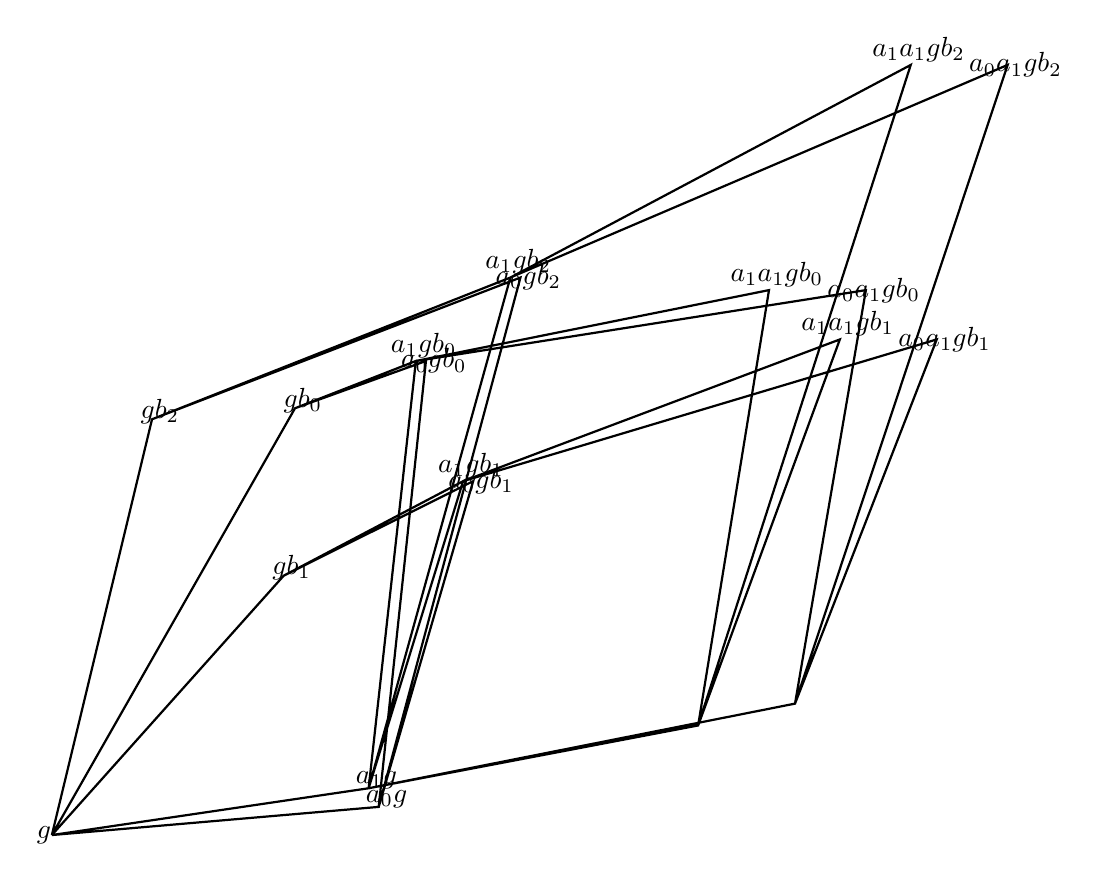
\begin{tikzpicture}
            \draw[thick](0,0)(0, 0) -- (3.088353468644447,5.4205516387976544) -- (4.750789476676656,6.020551638797654) -- (4.150789476676656,0.3576059661075695) -- (0, 0)
(0, 0) -- (2.9450115643433747,3.2943333900588665) -- (5.350789476676656,4.494333390058866) -- (4.150789476676656,0.3576059661075695) -- (0, 0)
(0, 0) -- (1.272049096589631,5.28032490810756) -- (5.950789476676656,7.08032490810756) -- (4.150789476676656,0.3576059661075695) -- (0, 0)
(0, 0) -- (3.088353468644447,5.4205516387976544) -- (4.6229597966340155,6.020551638797654) -- (4.022959796634016,0.5942041566224917) -- (0, 0)
(0, 0) -- (2.9450115643433747,3.2943333900588665) -- (5.222959796634016,4.494333390058866) -- (4.022959796634016,0.5942041566224917) -- (0, 0)
(0, 0) -- (1.272049096589631,5.28032490810756) -- (5.822959796634016,7.08032490810756) -- (4.022959796634016,0.5942041566224917) -- (0, 0)
(4.022959796634016, 0.5942041566224917) -- (4.6229597966340155,6.020551638797654) -- (10.3379144765194,6.9205516387976544) -- (9.4379144765194,1.6690739995734711) -- (4.022959796634016, 0.5942041566224917)
(4.022959796634016, 0.5942041566224917) -- (5.222959796634016,4.494333390058866) -- (11.2379144765194,6.294333390058866) -- (9.4379144765194,1.6690739995734711) -- (4.022959796634016, 0.5942041566224917)
(4.022959796634016, 0.5942041566224917) -- (5.822959796634016,7.08032490810756) -- (12.137914476519398,9.78032490810756) -- (9.4379144765194,1.6690739995734711) -- (4.022959796634016, 0.5942041566224917)
(4.022959796634016, 0.5942041566224917) -- (4.6229597966340155,6.020551638797654) -- (9.107455747512857,6.9205516387976544) -- (8.207455747512856,1.3917052304559332) -- (4.022959796634016, 0.5942041566224917)
(4.022959796634016, 0.5942041566224917) -- (5.222959796634016,4.494333390058866) -- (10.007455747512857,6.294333390058866) -- (8.207455747512856,1.3917052304559332) -- (4.022959796634016, 0.5942041566224917)
(4.022959796634016, 0.5942041566224917) -- (5.822959796634016,7.08032490810756) -- (10.907455747512856,9.78032490810756) -- (8.207455747512856,1.3917052304559332) -- (4.022959796634016, 0.5942041566224917)
;
\node at (4.850789476676655,6.020551638797654) {$ a_{ 0  } gb_{ 0 } $};
\node at (5.450789476676656,4.494333390058866) {$ a_{ 0  } gb_{ 1 } $};
\node at (6.0507894766766555,7.08032490810756) {$ a_{ 0  } gb_{ 2 } $};
\node at (4.722959796634015,6.220551638797654) {$ a_{ 1  } gb_{ 0 } $};
\node at (5.322959796634016,4.694333390058866) {$ a_{ 1  } gb_{ 1 } $};
\node at (5.922959796634015,7.28032490810756) {$ a_{ 1  } gb_{ 2 } $};
\node at (10.4379144765194,6.9205516387976544) {$ a_{ 0  } a_{ 1 }gb_{ 0 } $};
\node at (11.3379144765194,6.294333390058866) {$ a_{ 0  } a_{ 1 }gb_{ 1 } $};
\node at (12.237914476519398,9.78032490810756) {$ a_{ 0  } a_{ 1 }gb_{ 2 } $};
\node at (9.207455747512856,7.120551638797655) {$ a_{ 1  } a_{ 1 }gb_{ 0 } $};
\node at (10.107455747512857,6.494333390058866) {$ a_{ 1  } a_{ 1 }gb_{ 1 } $};
\node at (11.007455747512855,9.980324908107558) {$ a_{ 1  } a_{ 1 }gb_{ 2 } $};
\node at (-0.1,0) {$ g $};
\node at (4.250789476676656,0.45760596610756954) {$ a_{ 0 }g $};
\node at (4.1229597966340155,0.6942041566224917) {$ a_{ 1 }g $};
\node at (3.188353468644447,5.520551638797654) {$ gb_{ 0 } $};
\node at (3.045011564343375,3.3943333900588666) {$ gb_{ 1 } $};
\node at (1.372049096589631,5.38032490810756) {$ gb_{ 2 } $};

            \end{tikzpicture}
            \end{center}
            \caption{Square of the complex, with edges $(g,ag), (agb, gb) \in E_A,
            (g,gb), (agb, ag) \in E_B.$ \label{fig:square}
            }
            \end{figure}
 \begin{figure}[H]
            %\label{fig:square}
            \begin{center}
            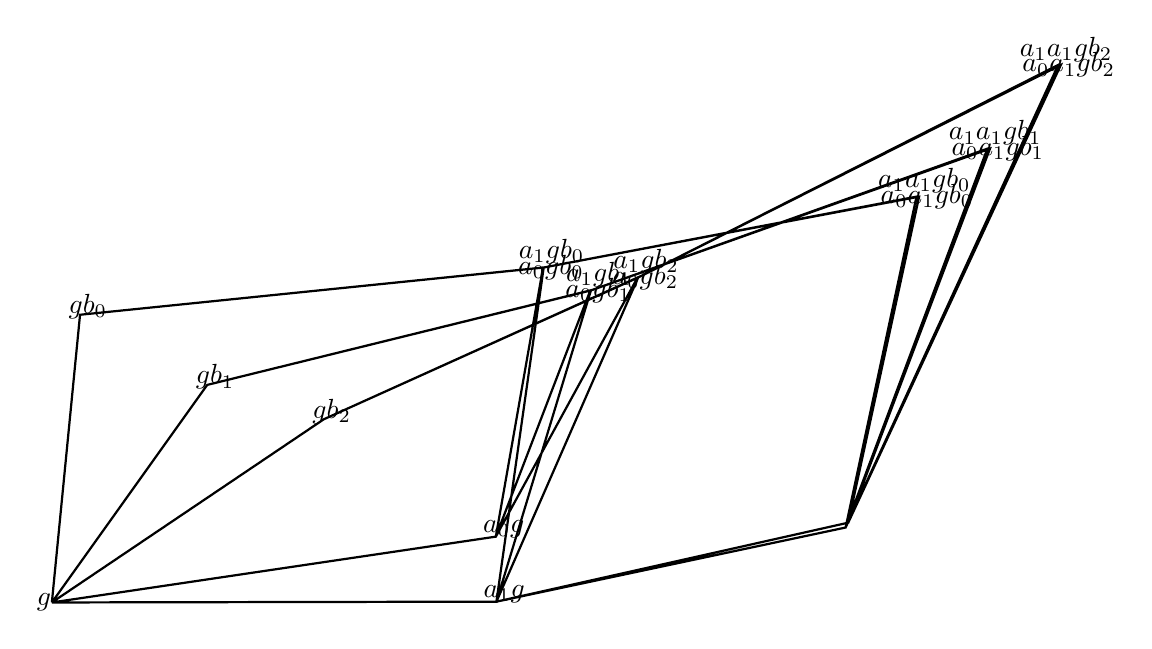
\begin{tikzpicture}
            \draw[thick](0,0)(0, 0) -- (0.35770069117497083,3.653696150324962) -- (6.238142051704713,4.253696150324962) -- (5.638142051704714,0.8358182898051959) -- (0, 0)
(0, 0) -- (1.9730334221860513,2.7629106604563023) -- (6.838142051704714,3.962910660456302) -- (5.638142051704714,0.8358182898051959) -- (0, 0)
(0, 0) -- (3.4535752058907794,2.3264241721870977) -- (7.438142051704713,4.126424172187098) -- (5.638142051704714,0.8358182898051959) -- (0, 0)
(0, 0) -- (0.35770069117497083,3.653696150324962) -- (6.245908778386146,4.253696150324962) -- (5.645908778386146,0.01018805874155948) -- (0, 0)
(0, 0) -- (1.9730334221860513,2.7629106604563023) -- (6.845908778386146,3.962910660456302) -- (5.645908778386146,0.01018805874155948) -- (0, 0)
(0, 0) -- (3.4535752058907794,2.3264241721870977) -- (7.445908778386146,4.126424172187098) -- (5.645908778386146,0.01018805874155948) -- (0, 0)
(5.645908778386146, 0.01018805874155948) -- (6.245908778386146,4.253696150324962) -- (11.013901073883195,5.153696150324962) -- (10.113901073883195,1.0133240428796104) -- (5.645908778386146, 0.01018805874155948)
(5.645908778386146, 0.01018805874155948) -- (6.845908778386146,3.962910660456302) -- (11.913901073883196,5.762910660456302) -- (10.113901073883195,1.0133240428796104) -- (5.645908778386146, 0.01018805874155948)
(5.645908778386146, 0.01018805874155948) -- (7.445908778386146,4.126424172187098) -- (12.813901073883194,6.826424172187098) -- (10.113901073883195,1.0133240428796104) -- (5.645908778386146, 0.01018805874155948)
(5.645908778386146, 0.01018805874155948) -- (6.245908778386146,4.253696150324962) -- (10.980590087193077,5.153696150324962) -- (10.080590087193077,0.9516936329074324) -- (5.645908778386146, 0.01018805874155948)
(5.645908778386146, 0.01018805874155948) -- (6.845908778386146,3.962910660456302) -- (11.880590087193077,5.762910660456302) -- (10.080590087193077,0.9516936329074324) -- (5.645908778386146, 0.01018805874155948)
(5.645908778386146, 0.01018805874155948) -- (7.445908778386146,4.126424172187098) -- (12.780590087193076,6.826424172187098) -- (10.080590087193077,0.9516936329074324) -- (5.645908778386146, 0.01018805874155948)
;
\node at (6.338142051704713,4.253696150324962) {$ a_{ 0  } gb_{ 0 } $};
\node at (6.938142051704713,3.962910660456302) {$ a_{ 0  } gb_{ 1 } $};
\node at (7.538142051704713,4.126424172187098) {$ a_{ 0  } gb_{ 2 } $};
\node at (6.345908778386145,4.453696150324962) {$ a_{ 1  } gb_{ 0 } $};
\node at (6.945908778386146,4.162910660456302) {$ a_{ 1  } gb_{ 1 } $};
\node at (7.545908778386146,4.326424172187098) {$ a_{ 1  } gb_{ 2 } $};
\node at (11.113901073883195,5.153696150324962) {$ a_{ 0  } a_{ 1 }gb_{ 0 } $};
\node at (12.013901073883195,5.762910660456302) {$ a_{ 0  } a_{ 1 }gb_{ 1 } $};
\node at (12.913901073883194,6.826424172187098) {$ a_{ 0  } a_{ 1 }gb_{ 2 } $};
\node at (11.080590087193077,5.3536961503249625) {$ a_{ 1  } a_{ 1 }gb_{ 0 } $};
\node at (11.980590087193077,5.962910660456302) {$ a_{ 1  } a_{ 1 }gb_{ 1 } $};
\node at (12.880590087193076,7.026424172187098) {$ a_{ 1  } a_{ 1 }gb_{ 2 } $};
\node at (-0.1,0) {$ g $};
\node at (5.738142051704713,0.9358182898051959) {$ a_{ 0 }g $};
\node at (5.745908778386146,0.11018805874155949) {$ a_{ 1 }g $};
\node at (0.4577006911749708,3.753696150324962) {$ gb_{ 0 } $};
\node at (2.073033422186051,2.8629106604563024) {$ gb_{ 1 } $};
\node at (3.5535752058907795,2.426424172187098) {$ gb_{ 2 } $};

            \end{tikzpicture}
            \end{center}
            \caption{Square of the complex, with edges $(g,ag), (agb, gb) \in E_A,
            (g,gb), (agb, ag) \in E_B.$ \label{fig:square}
            }
            \end{figure}
 \begin{figure}[H]
            %\label{fig:square}
            \begin{center}
            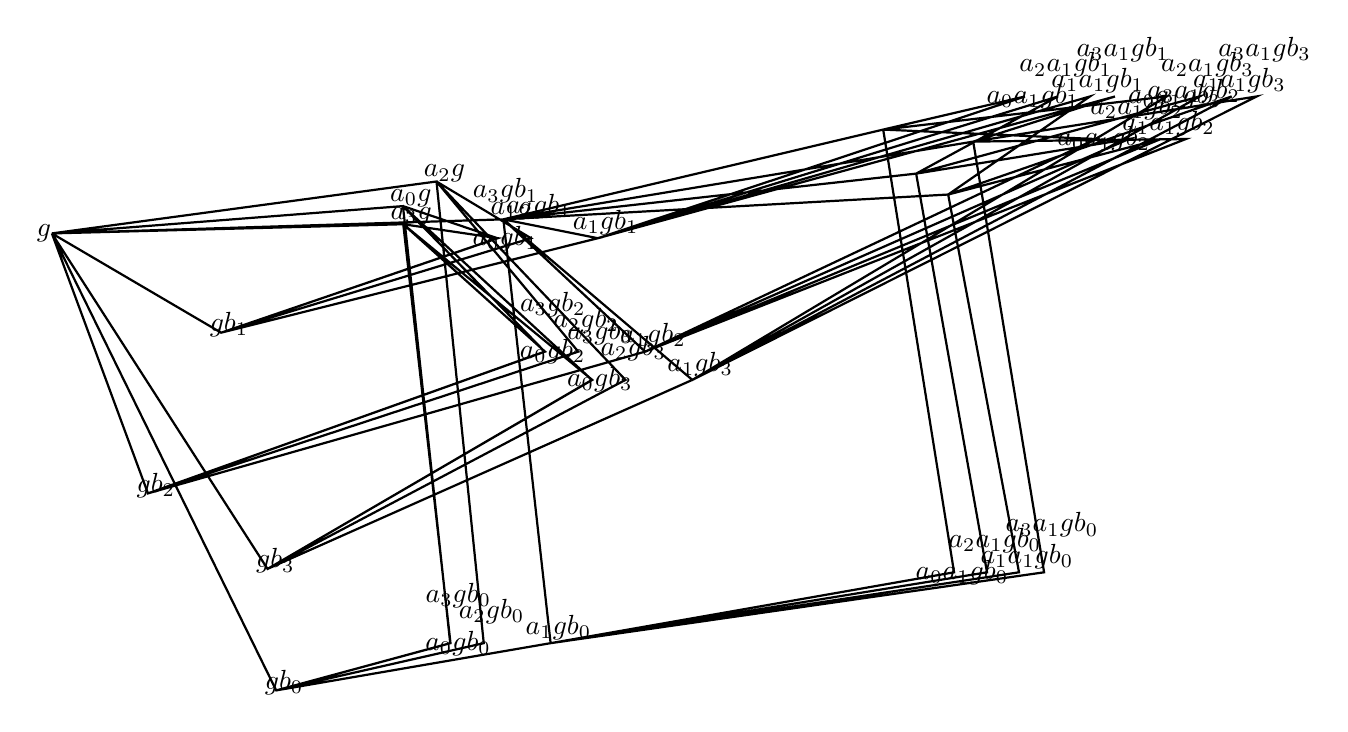
\begin{tikzpicture}
            \draw[thick](0,0)(0, 0) -- (2.849015370374231,-5.803799187378487) -- (5.058927132713739,-5.203799187378487) -- (4.45892713271374,0.3469246063114278) -- (0, 0)
(0, 0) -- (2.1495616343266017,-1.2609737943137564) -- (5.65892713271374,-0.06097379431375649) -- (4.45892713271374,0.3469246063114278) -- (0, 0)
(0, 0) -- (1.22047312342991,-3.3014513196752513) -- (6.2589271327137395,-1.5014513196752515) -- (4.45892713271374,0.3469246063114278) -- (0, 0)
(0, 0) -- (2.7388949536514176,-4.26050034507682) -- (6.85892713271374,-1.86050034507682) -- (4.45892713271374,0.3469246063114278) -- (0, 0)
(0, 0) -- (2.849015370374231,-5.803799187378487) -- (6.333902979758609,-5.203799187378487) -- (5.733902979758609,0.17861399796789137) -- (0, 0)
(0, 0) -- (2.1495616343266017,-1.2609737943137564) -- (6.933902979758609,-0.06097379431375649) -- (5.733902979758609,0.17861399796789137) -- (0, 0)
(0, 0) -- (1.22047312342991,-3.3014513196752513) -- (7.533902979758609,-1.5014513196752515) -- (5.733902979758609,0.17861399796789137) -- (0, 0)
(0, 0) -- (2.7388949536514176,-4.26050034507682) -- (8.13390297975861,-1.86050034507682) -- (5.733902979758609,0.17861399796789137) -- (0, 0)
(0, 0) -- (2.849015370374231,-5.803799187378487) -- (5.484821429914041,-5.203799187378487) -- (4.884821429914042,0.659336914626821) -- (0, 0)
(0, 0) -- (2.1495616343266017,-1.2609737943137564) -- (6.084821429914042,-0.06097379431375649) -- (4.884821429914042,0.659336914626821) -- (0, 0)
(0, 0) -- (1.22047312342991,-3.3014513196752513) -- (6.684821429914042,-1.5014513196752515) -- (4.884821429914042,0.659336914626821) -- (0, 0)
(0, 0) -- (2.7388949536514176,-4.26050034507682) -- (7.284821429914041,-1.86050034507682) -- (4.884821429914042,0.659336914626821) -- (0, 0)
(0, 0) -- (2.849015370374231,-5.803799187378487) -- (5.06274389633369,-5.203799187378487) -- (4.4627438963336905,0.11661640487080373) -- (0, 0)
(0, 0) -- (2.1495616343266017,-1.2609737943137564) -- (5.662743896333691,-0.06097379431375649) -- (4.4627438963336905,0.11661640487080373) -- (0, 0)
(0, 0) -- (1.22047312342991,-3.3014513196752513) -- (6.26274389633369,-1.5014513196752515) -- (4.4627438963336905,0.11661640487080373) -- (0, 0)
(0, 0) -- (2.7388949536514176,-4.26050034507682) -- (6.86274389633369,-1.86050034507682) -- (4.4627438963336905,0.11661640487080373) -- (0, 0)
(5.733902979758609, 0.17861399796789137) -- (6.333902979758609,-5.203799187378487) -- (11.457792513997516,-4.303799187378487) -- (10.557792513997516,1.3186483738568089) -- (5.733902979758609, 0.17861399796789137)
(5.733902979758609, 0.17861399796789137) -- (6.933902979758609,-0.06097379431375649) -- (12.357792513997516,1.7390262056862436) -- (10.557792513997516,1.3186483738568089) -- (5.733902979758609, 0.17861399796789137)
(5.733902979758609, 0.17861399796789137) -- (7.533902979758609,-1.5014513196752515) -- (13.257792513997515,1.1985486803247487) -- (10.557792513997516,1.3186483738568089) -- (5.733902979758609, 0.17861399796789137)
(5.733902979758609, 0.17861399796789137) -- (8.13390297975861,-1.86050034507682) -- (14.157792513997515,1.73949965492318) -- (10.557792513997516,1.3186483738568089) -- (5.733902979758609, 0.17861399796789137)
(5.733902979758609, 0.17861399796789137) -- (6.333902979758609,-5.203799187378487) -- (12.282845490188985,-4.303799187378487) -- (11.382845490188984,0.49364853403966447) -- (5.733902979758609, 0.17861399796789137)
(5.733902979758609, 0.17861399796789137) -- (6.933902979758609,-0.06097379431375649) -- (13.182845490188985,1.7390262056862436) -- (11.382845490188984,0.49364853403966447) -- (5.733902979758609, 0.17861399796789137)
(5.733902979758609, 0.17861399796789137) -- (7.533902979758609,-1.5014513196752515) -- (14.082845490188983,1.1985486803247487) -- (11.382845490188984,0.49364853403966447) -- (5.733902979758609, 0.17861399796789137)
(5.733902979758609, 0.17861399796789137) -- (8.13390297975861,-1.86050034507682) -- (14.982845490188984,1.73949965492318) -- (11.382845490188984,0.49364853403966447) -- (5.733902979758609, 0.17861399796789137)
(5.733902979758609, 0.17861399796789137) -- (6.333902979758609,-5.203799187378487) -- (11.876244129929933,-4.303799187378487) -- (10.976244129929933,0.7593097579526531) -- (5.733902979758609, 0.17861399796789137)
(5.733902979758609, 0.17861399796789137) -- (6.933902979758609,-0.06097379431375649) -- (12.776244129929934,1.7390262056862436) -- (10.976244129929933,0.7593097579526531) -- (5.733902979758609, 0.17861399796789137)
(5.733902979758609, 0.17861399796789137) -- (7.533902979758609,-1.5014513196752515) -- (13.676244129929934,1.1985486803247487) -- (10.976244129929933,0.7593097579526531) -- (5.733902979758609, 0.17861399796789137)
(5.733902979758609, 0.17861399796789137) -- (8.13390297975861,-1.86050034507682) -- (14.576244129929933,1.73949965492318) -- (10.976244129929933,0.7593097579526531) -- (5.733902979758609, 0.17861399796789137)
(5.733902979758609, 0.17861399796789137) -- (6.333902979758609,-5.203799187378487) -- (12.60110574345583,-4.303799187378487) -- (11.70110574345583,1.1659962500210885) -- (5.733902979758609, 0.17861399796789137)
(5.733902979758609, 0.17861399796789137) -- (6.933902979758609,-0.06097379431375649) -- (13.501105743455831,1.7390262056862436) -- (11.70110574345583,1.1659962500210885) -- (5.733902979758609, 0.17861399796789137)
(5.733902979758609, 0.17861399796789137) -- (7.533902979758609,-1.5014513196752515) -- (14.40110574345583,1.1985486803247487) -- (11.70110574345583,1.1659962500210885) -- (5.733902979758609, 0.17861399796789137)
(5.733902979758609, 0.17861399796789137) -- (8.13390297975861,-1.86050034507682) -- (15.30110574345583,1.73949965492318) -- (11.70110574345583,1.1659962500210885) -- (5.733902979758609, 0.17861399796789137)
;
\node at (5.158927132713739,-5.203799187378487) {$ a_{ 0  } gb_{ 0 } $};
\node at (5.7589271327137395,-0.06097379431375649) {$ a_{ 0  } gb_{ 1 } $};
\node at (6.358927132713739,-1.5014513196752515) {$ a_{ 0  } gb_{ 2 } $};
\node at (6.95892713271374,-1.86050034507682) {$ a_{ 0  } gb_{ 3 } $};
\node at (6.433902979758608,-5.003799187378487) {$ a_{ 1  } gb_{ 0 } $};
\node at (7.033902979758609,0.13902620568624352) {$ a_{ 1  } gb_{ 1 } $};
\node at (7.633902979758608,-1.3014513196752515) {$ a_{ 1  } gb_{ 2 } $};
\node at (8.233902979758609,-1.66050034507682) {$ a_{ 1  } gb_{ 3 } $};
\node at (5.584821429914041,-4.803799187378487) {$ a_{ 2  } gb_{ 0 } $};
\node at (6.184821429914042,0.33902620568624353) {$ a_{ 2  } gb_{ 1 } $};
\node at (6.784821429914041,-1.1014513196752516) {$ a_{ 2  } gb_{ 2 } $};
\node at (7.384821429914041,-1.4605003450768201) {$ a_{ 2  } gb_{ 3 } $};
\node at (5.16274389633369,-4.6037991873784865) {$ a_{ 3  } gb_{ 0 } $};
\node at (5.76274389633369,0.5390262056862436) {$ a_{ 3  } gb_{ 1 } $};
\node at (6.36274389633369,-0.9014513196752514) {$ a_{ 3  } gb_{ 2 } $};
\node at (6.96274389633369,-1.26050034507682) {$ a_{ 3  } gb_{ 3 } $};
\node at (11.557792513997516,-4.303799187378487) {$ a_{ 0  } a_{ 1 }gb_{ 0 } $};
\node at (12.457792513997516,1.7390262056862436) {$ a_{ 0  } a_{ 1 }gb_{ 1 } $};
\node at (13.357792513997515,1.1985486803247487) {$ a_{ 0  } a_{ 1 }gb_{ 2 } $};
\node at (14.257792513997515,1.73949965492318) {$ a_{ 0  } a_{ 1 }gb_{ 3 } $};
\node at (12.382845490188984,-4.1037991873784865) {$ a_{ 1  } a_{ 1 }gb_{ 0 } $};
\node at (13.282845490188985,1.9390262056862435) {$ a_{ 1  } a_{ 1 }gb_{ 1 } $};
\node at (14.182845490188983,1.3985486803247487) {$ a_{ 1  } a_{ 1 }gb_{ 2 } $};
\node at (15.082845490188983,1.93949965492318) {$ a_{ 1  } a_{ 1 }gb_{ 3 } $};
\node at (11.976244129929933,-3.9037991873784867) {$ a_{ 2  } a_{ 1 }gb_{ 0 } $};
\node at (12.876244129929933,2.1390262056862435) {$ a_{ 2  } a_{ 1 }gb_{ 1 } $};
\node at (13.776244129929934,1.5985486803247486) {$ a_{ 2  } a_{ 1 }gb_{ 2 } $};
\node at (14.676244129929932,2.13949965492318) {$ a_{ 2  } a_{ 1 }gb_{ 3 } $};
\node at (12.70110574345583,-3.7037991873784866) {$ a_{ 3  } a_{ 1 }gb_{ 0 } $};
\node at (13.60110574345583,2.3390262056862436) {$ a_{ 3  } a_{ 1 }gb_{ 1 } $};
\node at (14.50110574345583,1.7985486803247488) {$ a_{ 3  } a_{ 1 }gb_{ 2 } $};
\node at (15.40110574345583,2.33949965492318) {$ a_{ 3  } a_{ 1 }gb_{ 3 } $};
\node at (-0.1,0) {$ g $};
\node at (4.558927132713739,0.44692460631142783) {$ a_{ 0 }g $};
\node at (5.833902979758609,0.2786139979678914) {$ a_{ 1 }g $};
\node at (4.984821429914041,0.759336914626821) {$ a_{ 2 }g $};
\node at (4.56274389633369,0.21661640487080375) {$ a_{ 3 }g $};
\node at (2.949015370374231,-5.703799187378487) {$ gb_{ 0 } $};
\node at (2.249561634326602,-1.1609737943137564) {$ gb_{ 1 } $};
\node at (1.32047312342991,-3.201451319675251) {$ gb_{ 2 } $};
\node at (2.8388949536514176,-4.16050034507682) {$ gb_{ 3 } $};

            \end{tikzpicture}
            \end{center}
            \caption{Square of the complex, with edges $(g,ag), (agb, gb) \in E_A,
            (g,gb), (agb, ag) \in E_B.$ \label{fig:square}
            }
            \end{figure}
 
%\end{multicols*}
  % \printbibliography 
\end{document}

 